\documentclass[10pt,a4paper]{article}
\usepackage[utf8]{inputenc}
\usepackage{amsmath}
\usepackage{amsfonts}
\usepackage{amssymb}
\usepackage{graphicx}
\usepackage{hyperref}


\graphicspath{{img//}}

%\pagestyle{headings}

\author{Antonia Wagner \and Daniel Buth \and Johannes Müller \\ \\
Fachbereich Angewandte Informatik der Hochschule Fulda\\ \\
Modul \textit{Soft Computing}\\
Prof. Dr. Oleg Taraszow\\ \\
Betreuer: Lukas Militz
}
% Matrikel: Daniel: 128017, Antonia: 328213
\title{Fuzzygesteuerte U-Bahn Simulation}
\date{Wintersemester 2010/11}

\makeindex

\begin{document}

\maketitle

\includegraphics[scale=.3]{ubahnlogo}

\newpage 

\tableofcontents

\begin{abstract}
Diese Dokumentation beschreibt das Projekt \textit{FUZ-Bahn}, das wir im Praktikum zum Modul \textit{Soft Computing} im Wintersemester 2010/11 am Fachbereich Angewandte Informatik der Hochschule Fulda durchführten unter Betreung von Lukas Militz.
Zum Projektergebnis gehören eine fis-Datei der Fuzzy-Toolbox von Matlab sowie ein lauffähiges Java-Applet zu Visualisierung. Alle Ergebnisse inklusive Quellcode sowie diese Dokumentation sind über den Link \url{https://github.com/straight-shoota/FUZ-Bahn} auf der Online-Plattform Github zum Download verfügbar.
\end{abstract}

\newpage 

\section{Projektrahmen}
\subsection{Aufgabenstellung}
Unsere Aufgabenstellung war es, im Rahmen des Praktikums zur Lehrveranstaltung \textit{Soft Computing} bei Prof. Dr. Oleg Taraszow einen Fuzzy-Regler zu erstellen.
Als Werkzeug stand uns dazu die \textit{Fuzzy-Toolbox} der Software \textit{Matlab} zur Verfügung.
Optionale Bonusaufgabe war die Erstellung eines Java-Applets zur Visualisierung.

\begin{figure}[htb]
\begin{itemize}
	\item Eingangsvariablen: mindestens 3, mindestens 15 Terme
	\item Ausgangsvariablen: mindestens 2, mindestens 8 Terme
	\item Regeln: mindestens 25
\end{itemize}
\caption{Projektvorgaben}
\label{projektvorgaben}
\end{figure}

\subsection{Projektrahmen}
Bei Bewegungen kommen an vielen Stellen unscharfe Werte vor wie beispielsweise Geschwindigkeit, Entfernungen und Veränderungen dieser Parameter. Daher wollten wir unser Projekt im Bereich Verkehr ansiedeln.
Eine der ersten größere Anwendungen eines Fuzzy-Reglers in der Praxis die automatisierte Anfahr--, Beschleunigungs-- und Bremssteuerung der U-Bahn Sendai in Japan und wir entschieden uns, ein ähnliches Konzept umzusetzen.

\begin{figure}[htb]
\begin{center}
\leavevmode
\includegraphics[width=.8\textwidth]{Sendai_subway_1014_20081021.jpg}
\caption[Sendai Subway]{Sendai Subway}
\label{Sendai Subway}

\begin{footnotesize}
Quelle: Wikimedia Commons, hochgeladen von Benutzer Jet-0
\url{http://commons.wikimedia.org/wiki/File:Sendai_subway_1014_20081021.jpg}
\end{footnotesize}

\end{center}
\end{figure}

Unser Projekt sollte die Fahr- und Bremssteuerung eines schienengebundenen Verkehrsmittels wie eine U-Bahn mittels Fuzzy-Logic umsetzen.
Im Gegensatz zum Pionierprojekt der U-Bahn Sendai wollten wir jedoch eine komplette Fahrzeugsteuerung mittels Fuzzy-Regler erreichen.
\paragraph{}
Durch unseren Regler sollte das gesteuerte Fahrzeug in der Lage sein, aus dem Stillstand anzufahren und bis zu einer bestimmten, festgesetzten Geschwindigkeit zu beschleunigen und diese zu halten. Bei auf der Strecke voraus liegenden Wegpunkten wie eine Haltestelle oder ein Signal mit Haltbegriff soll ein Bremsvorgang eingeleitet werden, der das Fahrzeug möglichst sanft und punktgenau zum Stehen bringt.
\paragraph{}
Ebenso sollte es möglich sein, eine beliebige Geschwindigkeit erreichen und halten zu können. Dies kann beispielsweise bei einem langsameren vorausfahrenden Fahrzeug nötig sein. Auch die Einrichtung einer Langsamfahrstrecke kann ein solches Verhalten erfordern.
\paragraph{}
Zusätzlich zur eigentlichen Projektaufgabe haben wir uns zudem als Ziel gesetzt, als Bonusaufgabe eine Anwendung unseres Reglers als Java-Applet zu realisieren.

\section{Vorüberlegungen}
\subsection{Szenario}

Um das Projekt überschaubar zu halten, beschränkten wir unser Szenario auf den ganz einfachen Fall eines linearen, ebenen Streckenverlaufs ohne Abzweigungen oder sonstige andersgeartete Einflüsse. Auf dieser Strecke können sich einzig Hindernisse wie Haltestellen, vorausfahrende Züge oder Geschwindigkeitsbegrenzungen befinden. Das Fahrzeug sollte nur in der Lage sein, vorwärts zu fahren, sowie Beschleunigungs-- und Bremsvorgänge auszuführen. Ein Fahrtrichtungswechsel ist nicht vorgesehen.

\subsection{Fuzzy-Regler}

\subsubsection{Eingangsvariablen}
Als Eingangsvariablen wählten wir zunächst die einfachen Fahrzeugparameter der aktuellen Geschwindigkeit sowie die Entfernung zum nächsten Hindernis. Diese Variablen allein würden schon genügen, um ein einfaches Stop-and-Go-Verhalten zu erreichen, bei dem das Fahrzeug an jedem Punkt auf seinem Weg anhält um dann ggf. wieder neu anzufahren.
\newline
Dies reichte uns allerdings nicht aus, da auch die Geschwindigkeitskomponente des Zielobjektes berücksichtigt werden sollte, wenn es sich um einen vorausfahrendes Fahrzeug handelt oder eine Geschwindigkeitsbegrenzung erreicht werden soll.
Die Verarbeitung der konkreten Geschwindigkeit des Zielobjekts im Regler würde allerdings zu einer unüberschaubaren Fülle an Kombinationen von aktueller und zu erreichender Geschwindigkeit führen. Daher führten wir stattdessen den Geschwindigkeitsunterschied als Differenz von Zielgeschwindigkeit und aktueller Fahrzeuggeschwindigkeit als Variable ein.
\paragraph{Wertebereiche}
Die aktuelle Geschwindigkeit beträgt mindestens $ 0\, km/h $. Als zulässige Streckenhöchstgeschwindigkeit legten wir U-Bahn-typische $ 80\, km/h $ fest, um auch leichte Überläufe erlauben zu können, vergrößerten wir den Wertebereich allerdings noch um ein gutes Stück auf $ 120\, km/h $.

\begin{figure}[htb]
\begin{center}
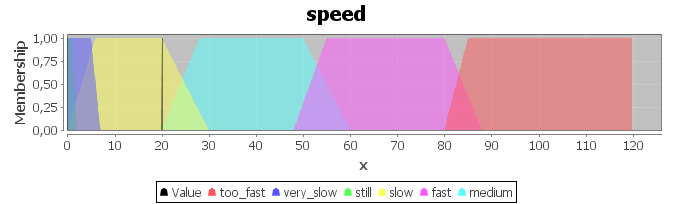
\includegraphics[width=\textwidth]{var_speed.png}
\caption[Eingangsvariable Geschwindigkeit]{Terme der Eingangsvariable Geschwindigkeit}
\label{var_speed}
\end{center}
\end{figure}

Den Wertebereich für die Entfernung des Ziels legten wir fest auf den Bereich von $ 0 - 1500 \, m $ wodurch ein genügend weiter Ausblick auf die vor dem Zug liegende Strecke gewährleistet ist.

\begin{figure}[htb]
\begin{center}
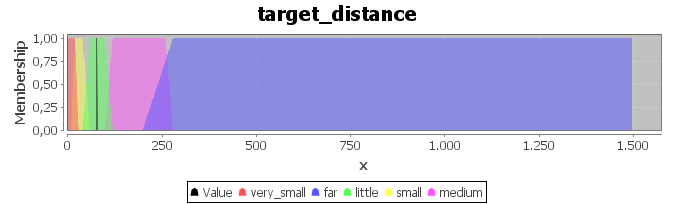
\includegraphics[width=\textwidth]{var_target_distance.png}
\caption[Eingangsvariable Zielentfernung]{Terme der Eingangsvariable Zielentfernung}
\label{var_target_distance}
\end{center}
\end{figure}

Analog zur aktuellen Geschwindigkeit liegt die Geschwindigkeitsdifferenz zwischen der Höchstgeschwindigkeit und dem betragsgleichen negativen Wert.

\begin{figure}[htb]
\begin{center}
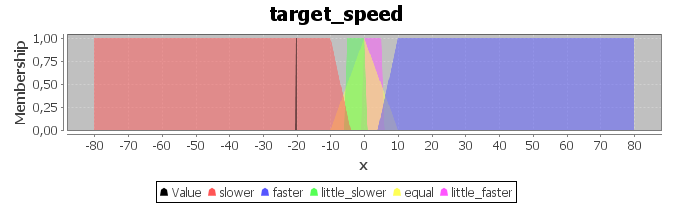
\includegraphics[width=\textwidth]{var_target_speed.png}
\caption[Eingangsvariable Geschwindigkeitsdifferenz]{Terme der Eingangsvariable Geschwindigkeitsdifferenz}
\label{var_target_speed}
\end{center}
\end{figure}

\subsubsection{Ausgangsvariablen}
Auf die Geschwindigkeit beziehungsweise die Beschleunigungsvorgänge eines elektrisch betriebenen Schienenfahrzeugs haben zwei Komponenten wesentlichen Einfluss: Der Fahrmotor sowie die Betriebsbremse (Druckluftbremse).
\paragraph{Zum Beschleunigen} wird die Leistung des Fahrmotors erhöht, wodurch elektrische Energie in Bewegungsenergie umgesetzt wird. Um eine Geschwindigkeit beizubehalten (Nullbeschleunigung) genügt es, den Fahrmotor für eine geringe Leistungsabgabe anzusteuern, da lediglich die durch die Bewegung verlorene Reibungsverluste ausgeglichen werden müssen. Wenn der Motor in den Leerlauf schaltet, sinkt die Geschwindigkeit kontinuierlich ab.

\begin{figure}[htb]
\begin{center}
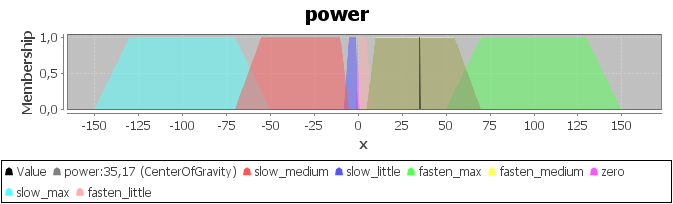
\includegraphics[width=\textwidth]{var_power.png}
\caption[Ausgangsvariable Motorleistung]{Terme der Ausgangsvariable Motorleistung}
\label{var_power}
\end{center}
\end{figure}

\paragraph{Beim Bremsen} (negative Beschleunigung) wirkt einerseits die Betriebsbremse, die je nach gewünschter Bremsstärke durch druckluftbetriebene Bremszylinder eine Bremskraft auf die Radachsen bewirkt. Im Regelbetrieb wird die zur Verfügung stehende Bremskraft nur zu einem Bruchteil beansprucht, volle Leistung wird nur bei einer Notbremsung abgerufen.

\begin{figure}[htb]
\begin{center}
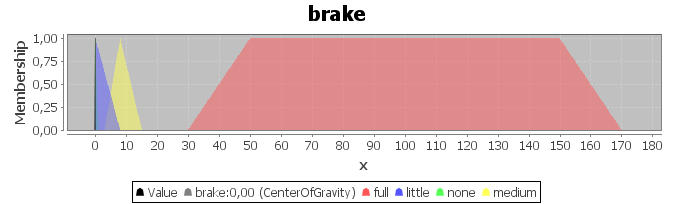
\includegraphics[width=\textwidth]{var_brake.png}
\caption[Ausgangsvariable Bremsstärke]{Terme der Ausgangsvariable Bremsstärke}
\label{var_brake}
\end{center}
\end{figure}

Zudem kommt beim Bremsen eine Besonderheit des Elektromotors zum Tragen: Die elektrische Bremswirkung, die eintritt, wenn ein Elektromotor in den Generatorbetrieb umgeschaltet wird. Dieser Vorteil einer stufenlosen und verschleißarmen Bremswirkung wird in der Praxis bei nahezu allen elektrischen Triebfahrzeugen eingesetzt, erreicht allerdings keine so starke Bremsbeschleunigung wir eine mechanische Bremse, weshalb diese stets zusätzlich vorhanden sein muss und bei stärkeren Bremsvorgängen additiv zugeschaltet wird.
Auf in der Praxis oftmals zusätzlich verwendete weitere Bremssysteme wurde im Zuge der Vereinfachung verzichtet.

\paragraph{Wertebereiche}
Als Wertebereiche verwendeten wir für die Motorsteuerung den Bereich $ -100 \% $ und $ +100 \% $ während die Bremsstärke zwischen $ 0 \% $ und $ 100 \% $ liegt.

%\paragraph{}
Damit waren die Projektvorgaben (siehe \hyperref[projektvorgaben]{Figure \ref*{projektvorgaben}}) erfüllt.

\section{Umsetzung}

\subsection{Fuzzy-Toolbox}

Die Fuzzy-Toolbox in MATLAB ist ein Werkzeug, um einen Regler zu erstellen und in einer graphischen Übersicht sehen zu können, ob in einer bestimmten Situation eine (bestimmte) Regel greift. Also ob ein erwarteter Output entsprechend dem Input erfolgt. In einer graphischen Umgebung können so Regeln erstellt und editiert, sowie das Greifen der Regeln überprüft werden.\\
In den folgenden Bildern sind die einzelnen Teilbereiche der Toolbox zu sehen, mit der die Regeln für den Controller erstellt wurden.

\begin{figure}[htb]
\leavevmode
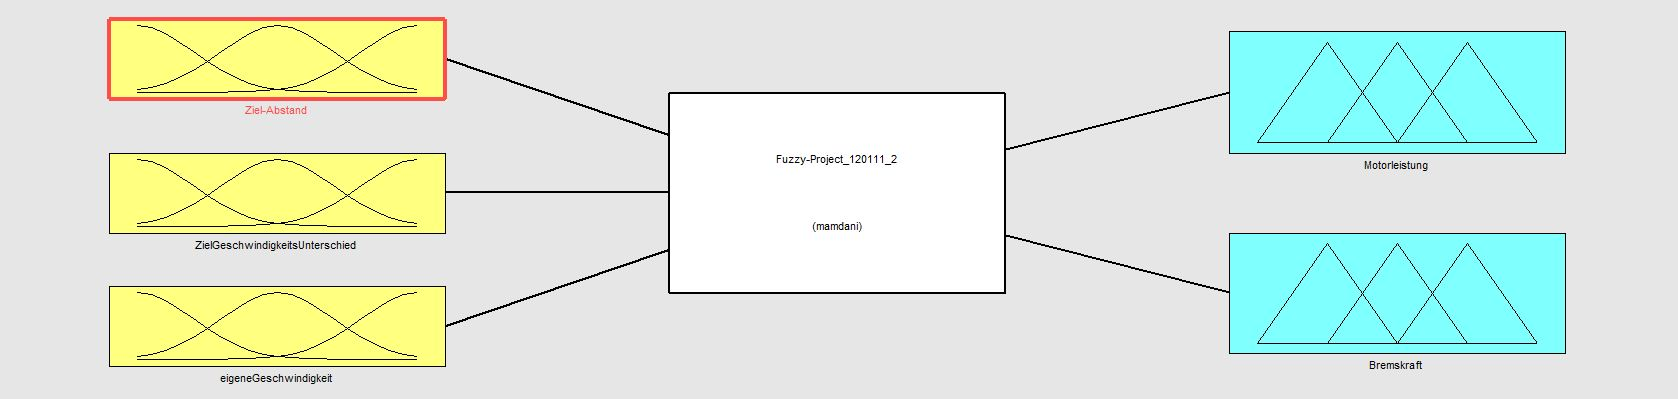
\includegraphics[width=\textwidth]{matlab1}
\caption[Hauptansicht]{Hauptansicht Fuzzy-Toolbox}
\label{matlab1}
\end{figure}

\begin{figure}[htb]
\leavevmode
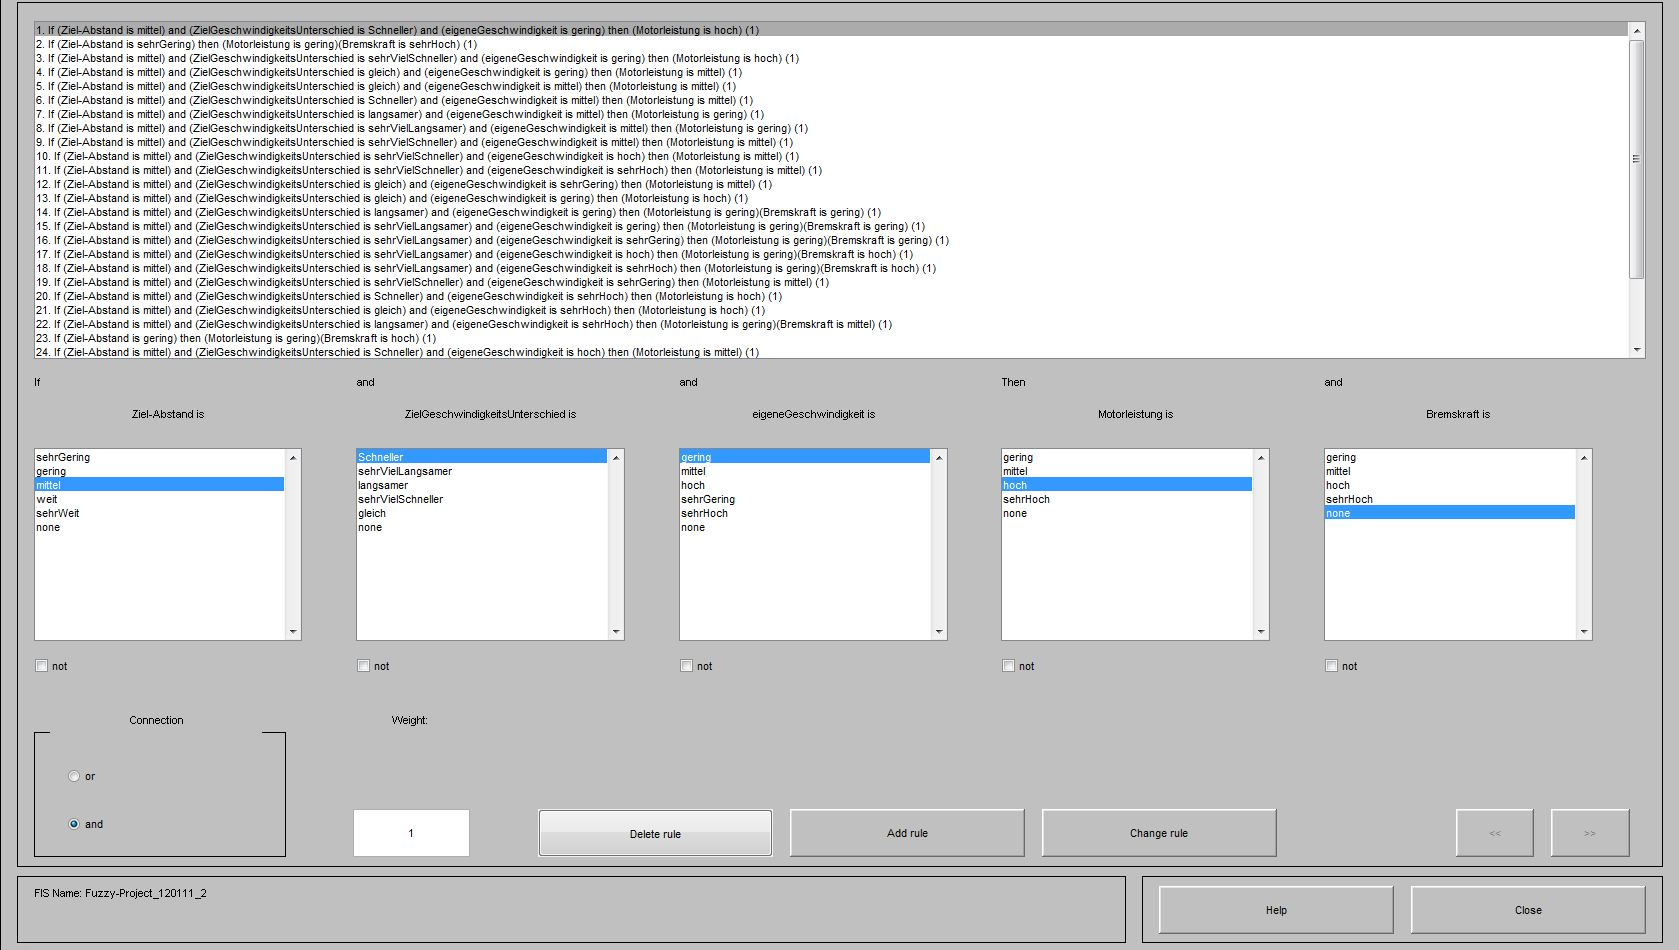
\includegraphics[width=\textwidth]{matlab_regeln}
\caption[Ansicht Regeln]{Regelansicht Fuzzy-Toolbox}
\label{matlab_regeln}
\end{figure}

\begin{figure}[htb]
\leavevmode
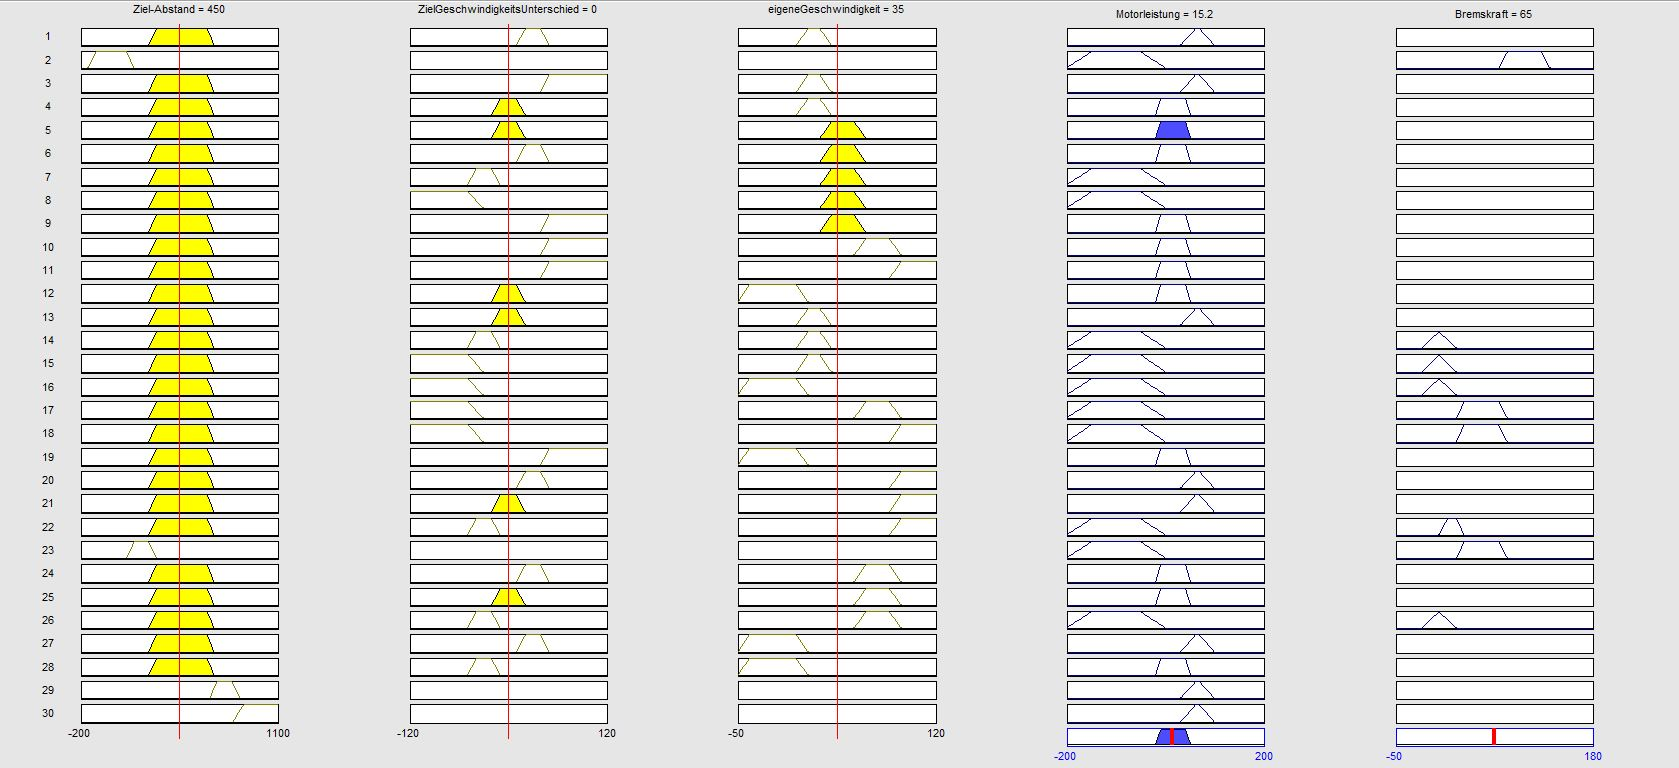
\includegraphics[width=\textwidth]{matlab_regeln_graphisch}
\caption[Ansicht Regeln (graphisch)]{Regelansicht Fuzzy-Toolbox, graphisch}
\label{matlab_regeln_graphisch}
\end{figure}

Die Regeln, die in MATLAB erstellt wurden und dann per Hand in das fcl-Format überführt wurden, waren mit dem Applet allerdings nicht lauffähig, sodass wir die Regeln erneut erstellten. Das zweite Mal verwendeten wir gleich das fcl-Format, um die Kompatibilität mit dem Applet gewährleisten und gleich testen zu können. Diese Regeln waren dann auch lauffähig.

\subsection{Applet}
Das Applet setzt die theoretischen Vorgaben in Programmcode und visuell um. Dabei werden die angegebenen Ausgangsvariablen überwacht und entsprechend der Regeln auf die gegebene Situation reagiert. \\
Ein Zug, der zu dicht auf seinen Vordermann auffährt, bremst ab und überwacht den Abstand, bis wieder beschleunigt werden kann. \\
Nähert sich der Zug einer Station, so bremst er rechtzeitig ab und hält an der Bahnsteigkante an.

\paragraph*{•}
Zur Fuzzy-Steuerung dient die Open-Source-Bibliothek jFuzzyLogic (\url{http://jfuzzylogic.sourceforge.net}), ferner werden die Diagramme von der ebenso unter der GPL lizensierten Chart-Bibliothek JFreeChart (\url{http://www.jfree.org/jfreechart/}).

Die graphischen Oberfläche ist mit Swing realisiert und in zwei Bereiche unterteilt. Der obere Bereich stellt graphisch die Situation dar. Der untere Teil zeigt die Werte der Eingangsvariablen und die zugehörigen Werte der Ausgangsvariablen, sowie das Szenario.\\
Das Szenario ist fest vorgeschrieben. Es beinhaltet eine Station, an der der Zug anhält. Des Weiteren gibt es Abschnitte, die eine Geschwindigkeitsbegrenzung des fahrenden Zugs vorsehen. Zusätzlich ist implementiert, dass zu einem vorausfahrenden Zuge ein Sicherheitsabstand eingehalten wird. \\
Der Zustand eines Beispiel-Szenario kann man im folgenden Bild sehen:

\begin{figure}[htb]
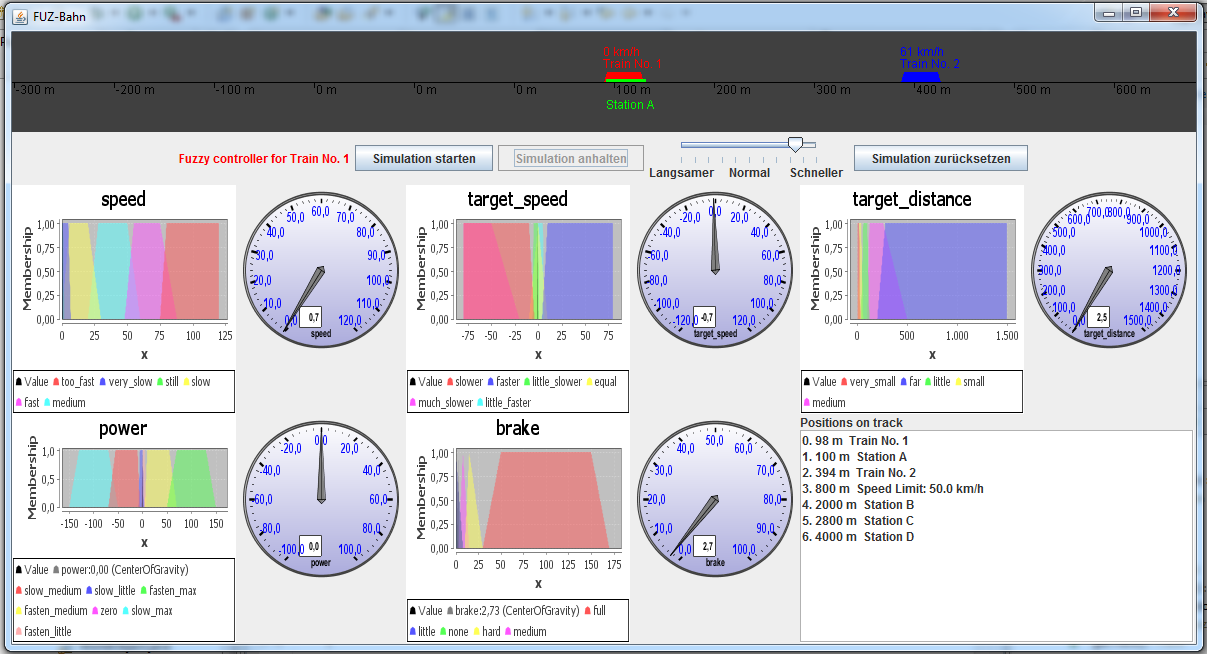
\includegraphics[width=\textwidth]{screenshot1}
\caption[Screenshot]{Screenshot der Java-Oberfläche zum Fuzzy-Regler: Zug hält an Station A}
\label{screenshot1}
\end{figure}

Die erste Reihen sind die Eingangsvariablen als Messwerte verschiedener Sensoren.
In der zweiten Reihe befinden sich die Ausgangsvariablen, die der Fuzzy-Regler anhand der vorgegebenen Regeln bestimmt.
Die simulierten Züge werden alle vom Fuzzy-Regler gesteuert, die Anzeigen gehören jeweils zum rot markierten "Train No. 1".
Neben den Ausgangsvariablen ist das Szenario als Liste dargestellt. Haltestellen und die Abschnitte mit Geschwindigkeitsbegrenzung sind im Programm als feste Teststrecke vorgegeben.
Wenn ein Zug eine Haltestelle oder einen Langsamfahrstrecke passiert, werden die Elemente, abhängig der Nähe zum Zug, entsprechend in der Liste "Positions on track" verschoben.\\ \\
Die Steuerung des Applets selbst wird in der Kopfleiste vorgenommen. Dort kann es gestartet, angehalten und zurückgesetzt werden.
Außerdem kann die Simulationsgeschwindigkeit hier geregelt werden.\\
Innerhalb der Simulation hält der Zug entsprechend Abstand zu dem voran fahrenden Fahrzeug. Je nach Geschwindigkeitsunterschied wird entsprechend auf die Situation reagiert. Ist der vordere Zug langsamer, bremst die Bahn, ist er schneller, kann ggf. beschleunigt werden, sofern keine Geschwindigkeitsbegrenzung in unmittelbarer Nähe vorliegt. \\
Diese theoretischen Vorgaben sind im Applet umgesetzt und der Regler hält sich daran. Dabei spielt es ebenfalls keine Rolle, wie viele Züge sich auf der Strecke befinden, der Regler erkennt dies und steuert alle Züge entsprechend der Situation.\\
Ist eine Geschwindigkeitsbegrenzung in unmittelbarer Nähe, gibt der Regler Signale an Bremse und Motor des Zugs, damit dieser entsprechend abbremst und an der Marke der Geschwindigkeitsbegrenzung die vorgegebene Geschwindigkeit, beispielsweise 50 km/h, einhält.\\
Befindet sich eine Haltestelle in Reichweite des Zuges, regelt der Controller das Abbremsen und Anhalten des Zuges und nachfolgend das erneute Anfahren und das Verhalten des Zuges auf den weiteren Streckenabschnitten.\\
Demzufolge sind alle wichtigen Eigenschaften, die eine einfach U-Bahnsimulation haben muss, erfüllt.

\subsubsection{Dynamikberechnungen}
\begin{equation}
E_{kin} = \frac{1}{2} m v^{2} 
\end{equation}

\begin{equation}
\bigtriangleup E = \bigtriangleup t \ast \bigtriangleup E
\end{equation}

\paragraph{Geschwindigkeit abhängig von Zeit und Energieveränderung}
\begin{equation}
E_{kin}(t_{1}) = E_{kin}(t_{2}) + \bigtriangleup t \ast P_{eff}
\end{equation}

\begin{equation}
v_{1} = \sqrt{v_{0}^2 + 2 \bigtriangleup t \frac{P_{eff}}{m}}
\end{equation}

\paragraph{Fahrwiderstände}

Zur Berechnung der Fahrwiderstände wurden jeweils die entsprechenden Grundformeln, aber stark vereinfacht eingesetzt.

\begin{equation}
W_F = W_R + W_L
\end{equation}
Der Fahrwiderstand des Zuges besteht aus dem Rollwiderstand auf ebener und gerader Fahrbahn und dem Luftwiderstand.
\subparagraph{Rollwiderstand}
\begin{equation}
W_R = c_w \ast m * g \\
\end{equation}
mit $ c_w \approx 0.0015 $
\subparagraph{Luftwiderstand}
\begin{equation}
W_L = \frac{p_{Luft}}{2} * c_w * A * v^2
\end{equation}
mit $ A \approx 10 m^2 $ und $ p_{Luft} \approx 1.2 $

\subparagraph{Streckenwiderstände} konnten komplett außer acht gelassen werden, da unser Szenario nur eine gerade, ebene, linear trassierte Strecke vorsieht, und daher keine Steigungs--, Neigungs-- oder Krümmungswiderstände auftreten.

\subparagraph{Beschleunigungswiderstand}
\begin{equation}
W_B = m * a
\end{equation}

\paragraph{Traktionsleistung}
\begin{equation}
P_{eff} = \sum W * v
\end{equation}

\begin{figure}[htb]
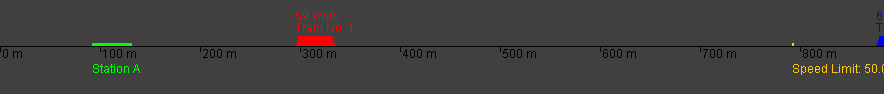
\includegraphics[width=\textwidth]{track}
\caption[Screenshot]{Ansicht der Gleisdarstellung}
\label{track}
\end{figure}

\subsubsection{Fahrzeugparameter}
Um die Berechnungen mit realistischen Werten durchführen zu können, erhielt unser Testfahrzeug typische Fahreigenschaften eines U-Bahn-Fahrzeugs. Insbesondere lehnten wir uns an die \textit{Baureihe B} der U-Bahn München, die bei der U-Bahn Nürnberg als Dt2 auch im Mischbetrieb mit automatisch gesteuerten Triebfahrzeugen verkehrt, und die \textit{Baureihe H} der U-Bahn Berlin an.

\begin{figure}[h]
\begin{center}
\begin{tabular}{|lr|}
\hline \textbf{Eigenschaft} & \textbf{Wert} \\ 
\hline Masse & $ 80\, t$ \\ 
\hline Länge & $ 40\, m$ \\ 
\hline Höchstgeschwindigkeit & $ 80 \, km/h $ \\ 
\hline Nennleistung & $ 780 \, kW $ \\ 
\hline maximale Bremskraft & $ 100 \, kN $ \\ 
\hline 
\end{tabular} 
\end{center}
\caption{Datenblatt unserer Testfahrzeugs}
\label{datenblatt}
\end{figure}

\section{Fazit}
Die Verwendung des in Matlab erzeugten Reglers erwies sich als schwieriges Unterfangen. Trotz Konvertierung in das von jFuzzyLogic verwendete FCL-Format brachte der Regler in der Java-Umgebung nicht die erwarteten Ergebnisse. Als Resultat blieb uns nichts anderes übrig, als die Regeln neu zu entwickeln und direkt in der Simulation live zu testen. Letztendlich kamen wir dabei dann sogar mit weniger Regeln gut zurecht.
Um die Projektvorgaben (siehe \hyperref[projektvorgaben]{Figure \ref*{projektvorgaben}}) jedoch einzuhalten, haben wir auch unsere ursprüngliche fis-Datei beibehalten.\\
Die Zusammenarbeit in der Gruppe hat gut funktioniert, es ist in unseren Augen ein vernünftiges Ergebnis entstanden. Von der Fuzzy-Toolbox waren wir allerdings ein wenig enttäuscht, da sie nicht sehr übersichtlich und schlecht bedienbar ist.\\
Die Dokumentation in der Gruppe war interessant; da es sich um eine wissenschaftliche Arbeit handelt, haben wir uns entschlossen, sie in Vorbereitung auf kommende Aufgaben wir die Bachlorthesis in \LaTeX zu schreiben, was auch gut geklappt hat.\\
Das Hauptproblem, auf das wir gestoßen sind, war, wie oben bereits genannt, die Tatsache, dass sich die vorgesehene Datei für den Fuzzy-Regler nicht verwenden ließ und wir mit den Regeln von vorne beginnen mussten.\\
Die Programmierung und Visualisierung hingegen waren nicht sehr problematisch, wenngleich nichts destotrotz auch aufwändig.

\end{document}